% !TEX root = ../main.tex
\subsection{CEBAF} \label{ssec::cebaf}
    \begin{figure}[htbp]
        \centering
        \fbox{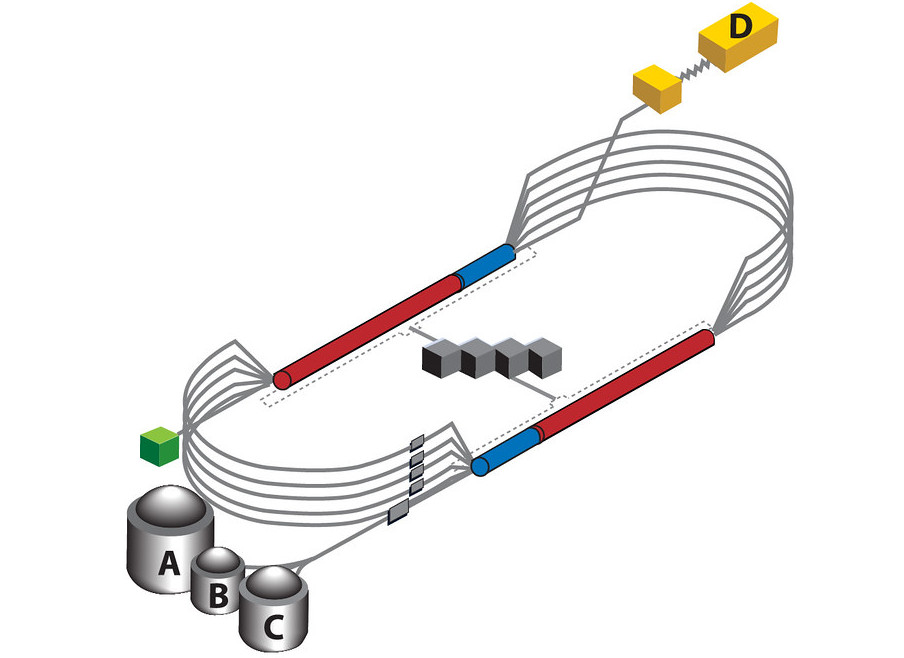
\includegraphics[width=0.8\textwidth]{11experiment/img/10cebaf.jpg}}
        \caption{\label{fig::cebaf} Schematic of CEBAF. \\
        Source: \texttt{https://www.flickr.com/photos/jeffersonlab/12599705145}}
    \end{figure}

    This document concerns work done at the Thomas Jefferson National Accelerator Facility (TJNAF) or Jefferson Laboratories (JLab) for short.
    Here, research is assisted by the use of one such linac, the Continuous Electron Beam Accelerator Facility (CEBAF).
    CEBAF is composed of a polarised electron source and a pair of two linacs connected through two arc sections.
    Electrons are accelerated via a pair superconducting magnets and guided through the arcs by steering magnets~\cite{leemann2001continuous}.

    The peculiar design of CEBAF allows for the continuous beam characteristic of other linacs, while also being able to reuse the tracks, effectively reaching energies found in an accelerator ten times its size~\cite{leemann2001continuous}.
    The electron beam can reach currents of a few nA, which corresponds to a luminosity of $\sim10^{34}$ $\text{cm}^{-2} \text{s}^{-1}$, and energies of up to 6 GeV (\textbf{TODO: PENDING CITATION}).

    A diagram of CEBAF can be seen in figure \ref{fig::cebaf}.

    After acceleration, the electron beam ends at one of the four available experiment halls, labelled by letters from A to D.
    Each contains a specialised spectrometer that records the products of collisions between the beam with itself or with a stationary target.
